\documentclass[twocolumn, 12pt]{article}

\usepackage[utf8]{inputenc}
\usepackage[english, spanish]{babel}
\usepackage{fullpage}
\usepackage{graphicx}
\usepackage{amsmath}
\usepackage{enumitem}
\usepackage{chngcntr}
\usepackage{setspace}
\usepackage{url}
\usepackage{csquotes}
\usepackage{float}
\usepackage{verbatim}
\usepackage{tabularx}
\usepackage{amsmath}
\usepackage{caption}

\counterwithin{figure}{section}
\renewcommand{\thesection}{\arabic{section}}
\renewcommand{\thesubsection}{\thesection.\arabic{subsection}}
\renewcommand{\baselinestretch}{1.5}

\usepackage[style=apa, maxnames=6, minnames=3, backend=biber]{biblatex}
\DefineBibliographyStrings{english}{%chktex-file 1 chktex-file 6
    andothers = {\em et\addabbrvspace al\adddot}
}
\addbibresource{./Bibliography/bibliography.bib}

\usepackage{array}
\usepackage{enumitem}

\setlength{\parskip}{0pt}

\raggedbottom{}

\begin{document}

\begin{titlepage}
    \centering
    
\includegraphics[width=0.3\textwidth]{Images/logo_utb.png}\par\vspace{1cm}
    {\scshape\LARGE Universidad Tecnológica de Bolívar \par}
    \vspace{1cm}

    {\scshape\Large FÍSICA ELÉCTRICA \par}
    \vspace{.2cm}

    % chktex-file 8
    {\scshape\Large H1 - C \par}
    \vspace{1cm}
    % chktex-file 8
    \slshape {\Large \bfseries{}Informe de Laboratorio No. VII\\}
    \vspace{1cm}

    \slshape {\itshape{} Mauro González, T00067622 \\}
    \slshape {\itshape{} German De Armas Castaño, T00068765 \\}
    \slshape {\itshape{} Angel Vega Rodriguez, T00068186 \\}
    \slshape {\itshape{} Juan Jose Osorio Ariza, T00067316 \\}
    \slshape {\itshape{} Juan Eduardo barón, T00065901 \\}
    \vfill
    Revisado Por \\
    Gabriel Hoyos Gomez Casseres\\
    {\large \today\par}
\end{titlepage}

% ----------------------------------------------------------------------|>
\section{Introducción}

Los circuitos eléctricos son sistemas cerrados de
componentes interconectados que permiten el flujo de
corriente eléctrica. Se dividen en circuitos de corriente
continua (CC) y circuitos de corriente alterna (CA),
dependiendo del flujo constante o periódico de la
corriente. La teoría de los circuitos eléctricos se ocupa
de analizar y comprender el comportamiento de estos
circuitos, basándose en principios fundamentales y leyes,
como las leyes de Kirchhoff.

Las leyes de Kirchhoff describen la conservación de la
carga y la energía en los circuitos eléctricos. La primera
ley establece que la suma de las corrientes que entran y
salen de un punto en un circuito cerrado es igual. La
segunda ley, conocida como la ley de mallas, establece que
la suma algebraica de las caídas de voltaje en las
resistencias alrededor de una trayectoria cerrada es igual
a la suma algebraica de las fuentes de voltaje en esa misma
trayectoria.

En este informe, analizaremos y verificaremos las leyes de
Kirchhoff utilizando valores experimentales, como
diferencias de potencial y corrientes. Estos análisis nos
permitirán comprender circuitos eléctricos más complejos,
donde múltiples componentes y fuentes de voltaje
interactúan entre sí.

% ----------------------------------------------------------------------|>
\section{Objetivos}

\subsection{Objetivo general}

\begin{itemize}[label=$\triangleright$]
    \item Explicar de manera clara y concisa las Leyes de Kirchhoff y
          su importancia en el análisis de circuitos eléctricos para
          así interpretar y sustentar de la mejor manera los cálculos
          realizados con sus respectivos resultados.
\end{itemize}

\subsection{Objetivos específicos}

\begin{itemize}[label=$\triangleright$]
    \item Detallar el fundamento teórico de las Leyes de Kirchhoff,
          incluyendo los principios de conservación de carga y
          energía en los circuitos eléctricos.
    \item Comprender el funcionamiento de un circuito eléctrico y
          como esto influye en el cálculo del voltaje.
    \item Discutir los conceptos y términos clave relacionados con
          las Leyes de Kirchhoff, como nodos, mallas, fuentes de
          voltaje, resistencias, corrientes y voltajes.
    \item Presentar los pasos y procedimientos para la resolución de
          problemas utilizando la ley de mallas y de nodos de
          Kirchhoff.
\end{itemize}

% ----------------------------------------------------------------------|>
\section{Marco Teórico}

% -------------------------------------------------------|>
\subsection{Leyes de Kirchhoff} \nocite{KhanAcademy__Kirchhoff}

% --------------------------------|>
\subsubsection{Ley de Corriente}

La ley de corriente de Kirchhoff establece que la suma
algebraica de todas las corrientes que convergen en un nodo
es igual a la suma algebraica de las corrientes que
divergen del nodo. Matemáticamente, se puede expresar de la
siguiente manera:

{\large
\begin{equation}
    \sum i_{adentro} = \sum i_{afuera}
\end{equation}
}

% --------------------------------|>
\subsubsection{Ley de Voltaje}

La suma de los voltajes alrededor de una malla es igual a
cero, lo cual se puede expresar mediante la ley de voltaje
de Kirchhoff de la siguiente manera:

En su forma general, considerando \textit{n} como el número
de voltajes de los componentes en la malla, se tiene:

{\large
\begin{equation}
    \sum v_n = 0
\end{equation}
}

Asimismo, la ley de voltaje de Kirchhoff se puede enunciar
de la siguiente manera: alrededor de una malla, la suma de
las subidas de voltaje es igual a la suma de las bajadas de
voltaje. Esto se expresa como:

{\large
\begin{equation}
    \sum v_{\text{subida}} = \sum v_{\text{bajada}}
\end{equation}
}

% ----------------------------------------------------------------------|>
\section{Montaje Experimental}

Para llevar a cabo el experimento en el laboratorio y
verificar las leyes de Kirchhoff, se emplearon distintos
elementos y materiales. Estos incluyeron alambres
conductores, un multímetro digital, dos fuentes de
corriente continua (D.C), cuatro resistores y un tablero
DINP\@.

Posteriormente, se procedió a montar el circuito siguiendo
un esquema diseñado específicamente para este propósito,
utilizando los materiales mencionados anteriormente.

\begin{figure}[H]
    \centering
    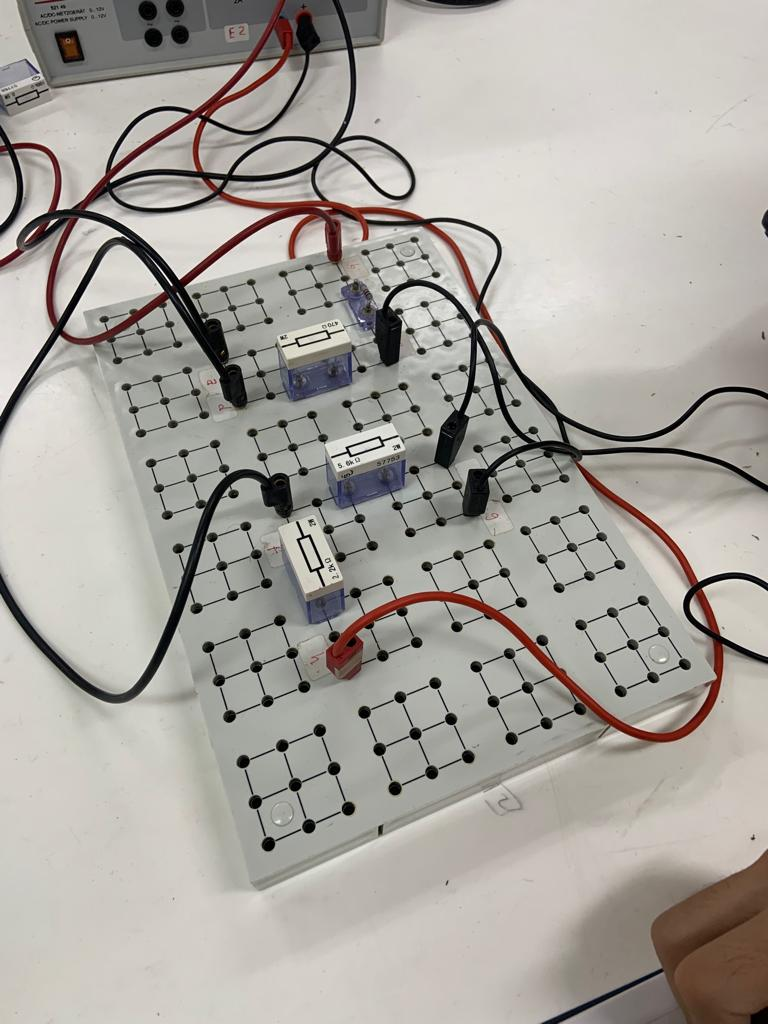
\includegraphics[width = 0.9\linewidth]{./Images/Imagen3.jpeg}
\end{figure}

\begin{figure}[H]
    \centering
    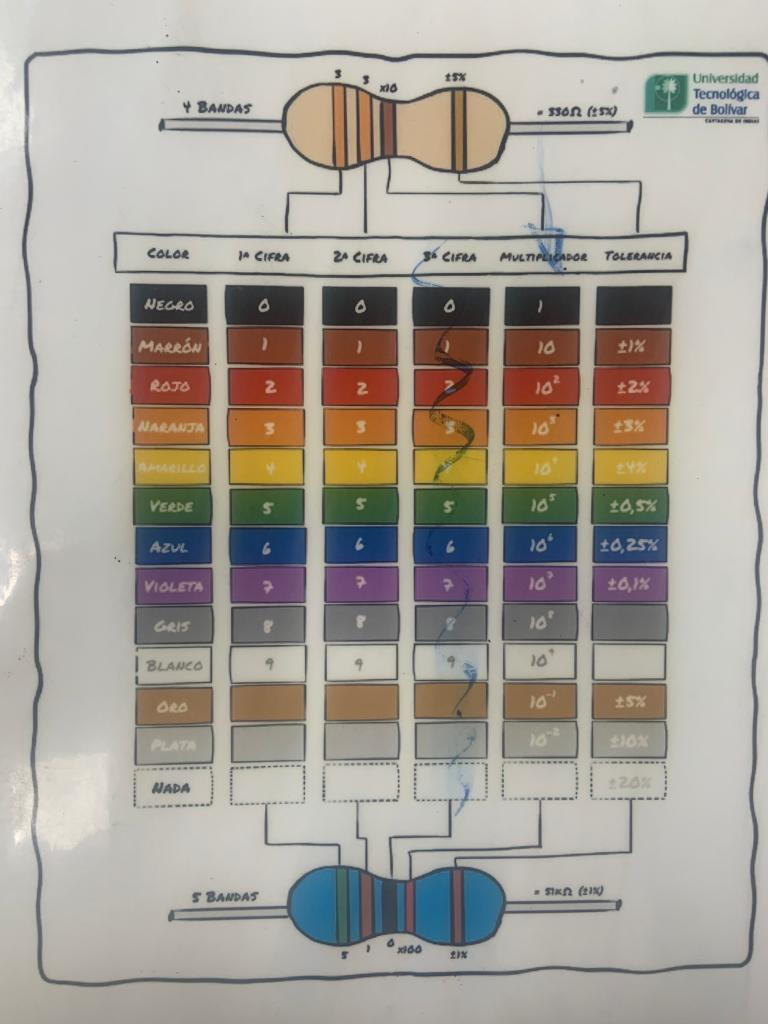
\includegraphics[width = 0.9\linewidth]{./Images/Imagen4.jpeg}
\end{figure}

% ----------------------------------------------------------------------|>
\section{Datos Experimentales}

\begin{table}[H]
    \captionsetup{justification=centering}
    \centering

    % chktex-file 44
    \begin{tabularx}{0.9\linewidth}{|>{\centering\arraybackslash}X|>{\centering\arraybackslash}X|>{\centering\arraybackslash}X|>{\centering\arraybackslash}X|}
        \multicolumn{4}{c}{Valor de resistencias $(K\Omega)$} \\ \hline

        $R_1$ & $R_2$  & $R_3$  & $R_4$                       \\ \hline
        $1$   & $0.47$ & $0.33$ & $2.2$                       \\ \hline
    \end{tabularx}

    \caption{Resistencia}

    % chktex-file 24
    \label{tab:datosExperimentales__Resistencias}
\end{table}

\vspace{.5cm}

\begin{table}[H]
    \captionsetup{justification=centering}
    \centering

    \begin{tabularx}{0.9\linewidth}{|>{\centering\arraybackslash}X|>{\centering\arraybackslash}X|>{\centering\arraybackslash}X|>{\centering\arraybackslash}X|>{\centering\arraybackslash}X|}
        \multicolumn{5}{c}{Valor de corrientes $(mA)$} \\ \hline

        $I_1$ & $I_2$ & $I_3$ & $I_4$ & $I_5$          \\ \hline
        $9.9$ & $3.6$ & $6.1$ & $0.5$ & $5.3$          \\ \hline
    \end{tabularx}

    \caption{Corriente}

    % chktex-file 24
    \label{tab:datosExperimentales__Corriente}
\end{table}

\vspace{.5cm}

\begin{table}[H]
    \captionsetup{justification=centering}
    \centering

    \begin{tabularx}{0.9\linewidth}{|>{\centering\arraybackslash}X|>{\centering\arraybackslash}X|>{\centering\arraybackslash}X|>{\centering\arraybackslash}X|}

        \multicolumn{4}{c}{Diferencias de potencial $(V)$}        \\ \hline
        $E1 \linebreak = B_{ab}$ & $V_{bc}$ & $V_{cd}$ & $V_{ef}$ \\ \hline
        $11.92$                  & $-10.06$ & $-1.86$  & $-1.8$   \\ \hline

        $E2 \linebreak = V_{gh}$ & $V_{hf}$ & $V_{ce}$ & \dots    \\ \hline
        $-0.45$                  & $-1.4$   & $0$      & \dots    \\ \hline
    \end{tabularx}

    \caption{Voltaje}

    % chktex-file 24
    \label{tab:datosExperimentales__DIFFPotencial}
\end{table}

\vspace{.5cm}

\begin{table}[H]
    \captionsetup{justification=centering}
    \centering

    \begin{tabularx}{0.9\linewidth}{|>{\centering\arraybackslash}X|>{\centering\arraybackslash}X|>{\centering\arraybackslash}X|>{\centering\arraybackslash}X|>{\centering\arraybackslash}X|}
        \multicolumn{5}{c}{Valor de corrientes $(mA)$} \\ \hline

        $I_1$  & $I_2$  & $I_3$ & $I_4$ & $I_5$        \\ \hline
        $9.98$ & $3.49$ & $5.9$ & $0.5$ & $5.6$        \\ \hline

    \end{tabularx}
    \caption{Corriente \textit{(FEM)}Invertida}

    % chktex-file 24
    \label{tab:datosExperimentales__Corriente-FEMInvertida}
\end{table}

% ----------------------------------------------------------------------|>
\section{Análisis de datos}

% -----------------------------------------------------|>
\subsection{Sume las diferencias de potencial en cada uno de los elementos del circuito para cada
    malla. Registre sus cálculos en la tabla 5.}

\begin{table}[H]
    \captionsetup{justification=centering}
    \centering

    \begin{tabularx}{0.9\linewidth}{|>{\centering\arraybackslash}X|>{\centering\arraybackslash}X|}
        \hline

        \textbf{Malla} & \textbf{V} \\\hline

    \end{tabularx}

    \begin{tabularx}{0.9\linewidth}{|>{\centering\arraybackslash}X|>{\centering\arraybackslash}X|}
        \hline
        $M_1$ \linebreak $[V_{ab} + V_{bc} + V_{cd}]$ &
        $= 11.92 - 10.05 - 1.86 = 0.01$ \linebreak
        $11.92 \simeq 11.91$                            \\ \hline
    \end{tabularx}

    \begin{tabularx}{0.9\linewidth}{|>{\centering\arraybackslash}X|>{\centering\arraybackslash}X|}
        \hline
        $M_2$ \linebreak $[V_{cd} + V_{ef}]$ &
        $= 1.86 - 1.8 = 0.06$ \linebreak
        $1.86 \simeq 1.8$                      \\\hline
    \end{tabularx}

    \begin{tabularx}{0.9\linewidth}{|>{\centering\arraybackslash}X|>{\centering\arraybackslash}X|}
        \hline
        $M_3$ \linebreak $[V_{gh} + V_{hf} + V_{ef}]$ &
        $= 0.45 - 1.4 + 1.8 = -0.05$ \linebreak
        $1.8 \simeq 1.85$                               \\ \hline
    \end{tabularx}

    \begin{tabularx}{0.9\linewidth}{|>{\centering\arraybackslash}X|>{\centering\arraybackslash}X|}
        \hline
        $A_{bgh}$ \linebreak $[V_{ab} + V_{bg} + V_{gh} + V_{ha}]$ &
        $= 11.92 - 10.06 + 0.45 - 1.81 = 0.5$ \linebreak
        $11.92 \simeq 11.87$                                         \\\hline
    \end{tabularx}

    \begin{tabularx}{0.9\linewidth}{|>{\centering\arraybackslash}X|>{\centering\arraybackslash}X|}
        \hline
        $A_{bef}$ \linebreak $[V_{ab} + V_{be} + V_{ef}]$ &
        $= 11.92 - 10.06 - 1.8 = -0.48$ \linebreak
        $11.92 \sim 12.4$                                   \\\hline
    \end{tabularx}

    \begin{tabularx}{0.9\linewidth}{|>{\centering\arraybackslash}X|>{\centering\arraybackslash}X|}
        \hline
        $A_{ghd}$ \linebreak $[V_{cg} + V_{gh} + V_{hd} + V_{dc}]$ &
        $= 0 + 0.45 - 1.8 + 1.86 = 0.51$ \linebreak
        $1.8 \sim 2.31$                                              \\\hline
    \end{tabularx}

    \caption{Diferencias de potencial}

    \label{tab:analisisDatos__1}
\end{table}

% -----------------------------------------------------|>
\subsection{¿Se cumple la ley de las mallas? ¿por qué?}

Si se verifica la ley de malla en un circuito, se observa
que los valores prácticos y teóricos concuerdan, aunque
pueda existir un pequeño error debido a la tolerancia
inherente de los elementos utilizados o a posibles
imprecisiones en los dispositivos de medición.

Es importante destacar que en ciertas ocasiones, este error
puede ser más evidente en ciertas partes del circuito, lo
cual puede requerir una consideración adicional para
evaluar con precisión el grado de coincidencia entre los
valores prácticos y teóricos.

% -----------------------------------------------------|>
\subsection{¿Si no resulta lo que se espera, a qué se deberá?}

Si los resultados obtenidos no son consistentes con las
expectativas, esto puede ser atribuido a diversos factores
de error, tales como mediciones inadecuadas, fallas en los
dispositivos utilizados o errores en los cálculos
realizados.

% -----------------------------------------------------|>
\subsection{¿Si realiza el recorrido en sentido contrario, también se cumple la ley de las mallas?
    ¿Cuál es la diferencia?}

La ley de la corriente de Kirchhoff establece que si se
cumple la conservación de carga en un nodo, la suma de las
corrientes que entran al nodo es igual a la suma de las
corrientes que salen del nodo. En caso de que no se cumpla
esta condición, las corrientes resultantes tendrán la misma
magnitud pero con signos opuestos para indicar la dirección
opuesta del flujo de corriente.

% -----------------------------------------------------|>
\subsection{¿Por qué $V_{ce}$ es cero?}

$V_{ce}$ es cero en un cable debido a que los extremos del cable
están directamente conectados, lo que implica que no hay
una diferencia de potencial significativa entre ellos. En
otras palabras, el voltaje en ambos extremos del cable es
igual pero con signos opuestos, lo cual resulta en un valor
de cero para Vce.

% -----------------------------------------------------|>
\subsection{Sume las corrientes que salen en cada nodo. Registre sus datos en la tabla 6}

Según los datos en la
tabla~\ref{tab:datosExperimentales__Corriente},

\begin{table}[H]
    \captionsetup{justification=centering}
    \centering

    \begin{tabularx}{0.9\linewidth}{|>{\centering\arraybackslash}X|>{\centering\arraybackslash}X|>{\centering\arraybackslash}X|}
        \hline
        \textbf{Nodo} & \textbf{Entra}               & \textbf{Sale}                \\\hline

        \textit{C}    & $I_1 = 9.9$                  & $I_2 + I_3 \linebreak = 9.7$ \\\hline

        \textit{E}    & $I_3 = 6.1$                  & $I_4 + I_5 \linebreak = 5.8$ \\\hline

        \textit{D}    & $I_4 + I_5 \linebreak = 5.8$ & $I_3 = 6.1$                  \\\hline

        \textit{F}    & $I_2 + I_3 \linebreak = 9.7$ & $I_1 = 9.9$                  \\\hline

    \end{tabularx}
    \caption{}

    \label{tab:analisisDatos__6}
\end{table}

% -----------------------------------------------------|>
\subsection{¿Se cumple la ley de los nodos? ¿Por qué?}

La ley de los nodos se cumple debido a que la suma de las
corrientes que entran a un nodo es igual a la suma de las
corrientes que salen del nodo

% -----------------------------------------------------|>
\subsection{¿Si no resulta lo que se espera, a qué se deberá?}

Si los resultados obtenidos difieren de lo esperado, esto
puede deberse a varios factores, como errores de medición,
fallas en los dispositivos utilizados, errores en los
cálculos o interpretación de los datos.

% -----------------------------------------------------|>
\subsection{Aplique las leyes de Kirchhoff para encontrar una expresión que nos permita calcular las
    corrientes en el circuito en términos de las resistencias y fem. Registre los resultados en
    la tabla 7}

Ver tabla~\ref{tab:analisisDatos__11}

% -----------------------------------------------------|>
\subsection{Calcule los valores de las corrientes remplazando en la expresión encontrada los valores
    de las resistencias y las fem (tabla 1 y 2). Registre los resultados en la tabla 7}

Ver tabla~\ref{tab:analisisDatos__11}

% -----------------------------------------------------|>
\subsection{Calcule la exactitud de la medida directa de las corrientes respecto a los valores teóricos
    encontrados por las leyes de Kirchhoff. Registre los resultados en la tabla 7. De una
    explicación a las causas de las diferencias en las medidas.}

\begin{table}[H]
    \captionsetup{justification=centering}
    \centering

    \begin{tabularx}{0.9\linewidth}{|>{\centering\arraybackslash}X|>{\centering\arraybackslash}X|>{\centering\arraybackslash}X|}
        \hline
        Expresión                  & I $(mA)$ Valor Teorico & I $(mA)$ Valor Medido \\\hline
        $I_1 = \frac{V_{bc}}{R_1}$ & $10.6$                 & $9.9$                 \\ \hline
        $I_2 = \frac{V_{cd}}{R_2}$ & $3.957$                & $3.6$                 \\ \hline
        $I_3 = I_4 + I_5$          & $5.8$                  & $6.1$                 \\ \hline
        $I_4 = I_3 - I_5$          & $0.8$                  & $0.5$                 \\ \hline
        $I_5 = \frac{V_{ef}}{R_3}$ & $5.4$                  & $5.3$                 \\ \hline
    \end{tabularx}

    \vspace{.2cm}

    \begin{tabularx}{0.9\linewidth}{|>{\centering\arraybackslash}X|>{\centering\arraybackslash}X|}
        \hline
        \multicolumn{2}{|c|}{Exactitud}                                                                       \\\hline
        \multicolumn{2}{|c|}{$1 - (\frac{ValorMedido - ValorTeorico}{ValorMedido + ValorTeorico}) \cdot 100$} \\\hline
        $I_1$ & $96\%$                                                                                        \\\hline
        $I_2$ & $95\%$                                                                                        \\\hline
        $I_3$ & $97\%$                                                                                        \\\hline
        $I_4$ & $76\%$                                                                                        \\\hline
        $I_5$ & $99\%$                                                                                        \\\hline
    \end{tabularx}

    \caption{}

    \label{tab:analisisDatos__11}
\end{table}

% -----------------------------------------------------|>
\subsection{Realice los procedimientos del 9 al 11, pero considerando la \textit{(FEM)} E2 invertida y los datos de la tabla 4}

\begin{table}[H]
    \captionsetup{justification=centering}
    \centering

    \begin{tabularx}{0.9\linewidth}{|>{\centering\arraybackslash}X|>{\centering\arraybackslash}X|>{\centering\arraybackslash}X|}
        \hline
        Expresión                  & I $(mA)$ Valor Teorico & I $(mA)$ Valor Medido \\\hline
        $I_1 = \frac{V_{bc}}{R_1}$ & $10.06$                & $9.98$                \\ \hline
        $I_2 = \frac{V_{cd}}{R_2}$ & $3.957$                & $3.49$                \\ \hline
        $I_3 = I_4 + I_5$          & $6.1$                  & $5.9$                 \\ \hline
        $I_4 = I_3 - I_5$          & $0.3$                  & $0.5$                 \\ \hline
        $I_5 = \frac{V_{ef}}{R_3}$ & $5.45$                 & $5.6$                 \\ \hline
    \end{tabularx}

    \vspace{.2cm}

    \begin{tabularx}{0.9\linewidth}{|>{\centering\arraybackslash}X|>{\centering\arraybackslash}X|}
        \hline
        \multicolumn{2}{|c|}{Exactitud}                                                                       \\\hline
        \multicolumn{2}{|c|}{$1 - (\frac{ValorMedido - ValorTeorico}{ValorMedido + ValorTeorico}) \cdot 100$} \\\hline
        $I_1$ & $99\%$                                                                                        \\\hline
        $I_2$ & $93\%$                                                                                        \\\hline
        $I_3$ & $98\%$                                                                                        \\\hline
        $I_4$ & $75\%$                                                                                        \\\hline
        $I_5$ & $98\%$                                                                                        \\\hline
    \end{tabularx}

    \caption{}

    \label{tab:analisisDatos__12}
\end{table}

% -----------------------------------------------------|>
\subsection{Observe todas las medidas que cambian (corrientes y diferencias de potencial) respecto
    al circuito inicial y de una explicación}

Las mediciones de corriente y diferencia de potencial
pueden variar según si se obtienen teóricamente o a través
de mediciones en el laboratorio. En experimentos de este
tipo, es común que las mediciones no sean completamente
precisas, lo que puede resultar en pequeñas variaciones en
los valores calculados. Al comparar los procedimientos para
el circuito normal y la inversión de la \textit{fem} E2,
observamos que los valores difieren significativamente.
Esta diferencia se debe a que la posición de la fem E2
afecta la corriente que fluye a través del circuito, lo que
a su vez afecta cada corriente en función de su trayectoria
con respecto a la fem posicionada de esa manera.

% -----------------------------------------------------|>
\subsection{Realice conclusiones y observaciones}

Las leyes de Kirchhoff desempeñan un papel fundamental en
el campo de la física eléctrica y son especialmente
relevantes en el estudio de circuitos eléctricos. Estas
leyes proporcionan un marco teórico para comprender el
comportamiento de las corrientes eléctricas y los voltajes
en estos sistemas. En este experimento, se construyó un
circuito eléctrico con el propósito de verificar de manera
práctica estas leyes, y se realizaron mediciones de
resistencia, voltaje e intensidad eléctrica.

Los resultados obtenidos concuerdan satisfactoriamente con
las predicciones teóricas, como se refleja en las tablas
correspondientes. Se observa que la corriente que entra en
cada nodo es casi igual a la corriente que sale de él, lo
cual es consistente con lo establecido por la ley de
Kirchhoff para los nodos. En conclusión, los resultados
experimentales obtenidos en el laboratorio son precisos,
como se evidencia en la alta exactitud de las mediciones en
comparación con los valores teóricos. Esto demuestra que
los valores medidos se ajustan a lo establecido por la
teoría de Kirchhoff. En consecuencia, se pudo llevar a cabo
y concluir de manera satisfactoria esta experiencia de
laboratorio relacionada con las leyes de Kirchhoff.

% ----------------------------------------------------------------------|>
\section{Conclusiones}

A lo largo del informe ``Circuitos de corriente eléctrica.
Leyes de Kirchhoff'', se llevó a cabo un análisis
exhaustivo, determinación, comprensión, aplicación y
explicación de las leyes de Kirchhoff, específicamente la
ley de las mallas y la ley de los nodos. Durante el
desarrollo del informe, se observó que la diferencia de
potencial en un circuito depende de la trayectoria que
sigue la corriente y de si el circuito está configurado en
serie o en paralelo. Además, se encontró que al
intercambiar el circuito de salida de una de las dos
fuentes electromotrices, las corrientes pueden variar, como
se evidencia en las tablas donde aumentan o disminuyen.

Mediante la aplicación de las leyes de Kirchhoff, se
obtuvieron expresiones que permitieron calcular las
corrientes en el circuito. En conclusión, las leyes de
Kirchhoff brindan una base sólida para el análisis y diseño
de diferentes tipos de circuitos eléctricos.

\printbibliography

\end{document}